\chapter{Running Example}
\label{ch:RunningExample}

The case study umljava provided in \cite{umljavacasestudy} serves as the running example.
It contains basic reactions code for preserving consistency in both directions, providing a good baseline for further expansion.
In addition to the reactions, the library example provides models of the real V-SUM that were used for testing and measurements.

\section{Reactions}
\label{sec:RunningExample:Reactions}

The first thing to consider is the actual reaction code and what can be built upon.
Existing reactions have been altered throughout this work by adding and adapting rules to fit the needs of derived configurations.

\lstinputlisting[frame=single, caption={Existing UML to Java reaction}, label=listing:existing-reaction, numbers=left, float=htbp, language=reactions]{examples/umlClassInserted.reactions}

\Autoref{listing:existing-reaction} shows an existing reaction that is responsible for creating or locating an existing Java class and connecting it to the newly created UML class.
Line one defines a new reaction called \textit{UmlClassInserted}.
The next line adds the trigger for this reaction, which starts the procedure when a new UML class is inserted.
The routines to execute are defined in the \textit{call} block and will be called when the reaction is triggered.

\lstinputlisting[frame=single, caption={Existing UML to Java routine}, label=listing:existing-routine, numbers=left, float=htbp, language=reactions]{examples/createOrFindJavaClass.reactions}

The routine definition for \textit{createOrFindJavaClass} is given in \autoref{listing:existing-routine}, which executes the actual logic with the help of Xtend code \cite{KLARE2021110815}.
The \textit{match} block ensures that this routine can be run, as it requires the absence of an existing Java class already linked to the UML class.
It also retrieves the optional Java package corresponding to the UML container in lines 4 \& 5.
This is used in the \textit{update} block, which can contain arbitrary Xtend code for creating files, changing packages, adding attributes, and so on.
This code can also call other routines and functions defined in Java.

\lstinputlisting[frame=single, caption={Routine calling a user interaction}, label=listing:external-method-call, numbers=left, float=htbp, language=reactions]{examples/propagateTypedMultiplicityElementTypeChanged.reactions}
\lstinputlisting[frame=single, caption={Existing user interaction}, label=listing:existing-user-interaction, numbers=left, float=htbp, language=Java]{examples/userSelectCollectionType.java}

One important functionality that remains to be examined is user interaction.
When a reaction has code for user interaction, the user is prompted with one of the possible dialogs, which they must complete to continue execution.
\Autoref{listing:external-method-call} is a routine that calls into code defined in Java, presenting the user with an interactive option.
In \autoref{listing:existing-user-interaction}, the user is asked what type of collection should be used on the Java side when the multiplicity on the UML side changes.
The result can then be used like any other variable in the code.
Expressing such a dialog in terms of features is left to \autoref{ch:FutureWork}.
Currently, the annotated reactions still contain it, so it remains a runtime decision in every derived configuration.
For now, a predefined selection is used, with the first option chosen in automatic runs.

Further reactions need to be added to enable variability and allow annotations to choose which features to use.
If a new UML class is to be modelled as a Java interface, the methodologist must create this new reaction, which can then be selected by the annotation representing the feature.
The case study also includes tests written in xtend to verify the behavior of its reactions.
These are extended to cover the new features and configurations, as described in \autoref{sec:Implementation:Testing}.

\section{Features and configurations}
\label{sec:RunningExample:FeaturesAndConfigurations}

One of the created artifacts is a feature model that defines the relationship between all features.
This is necessary so that the methodologist knows which configurations are valid.
The full model contains 37 features.

\begin{sidewaysfigure}
    \centering
    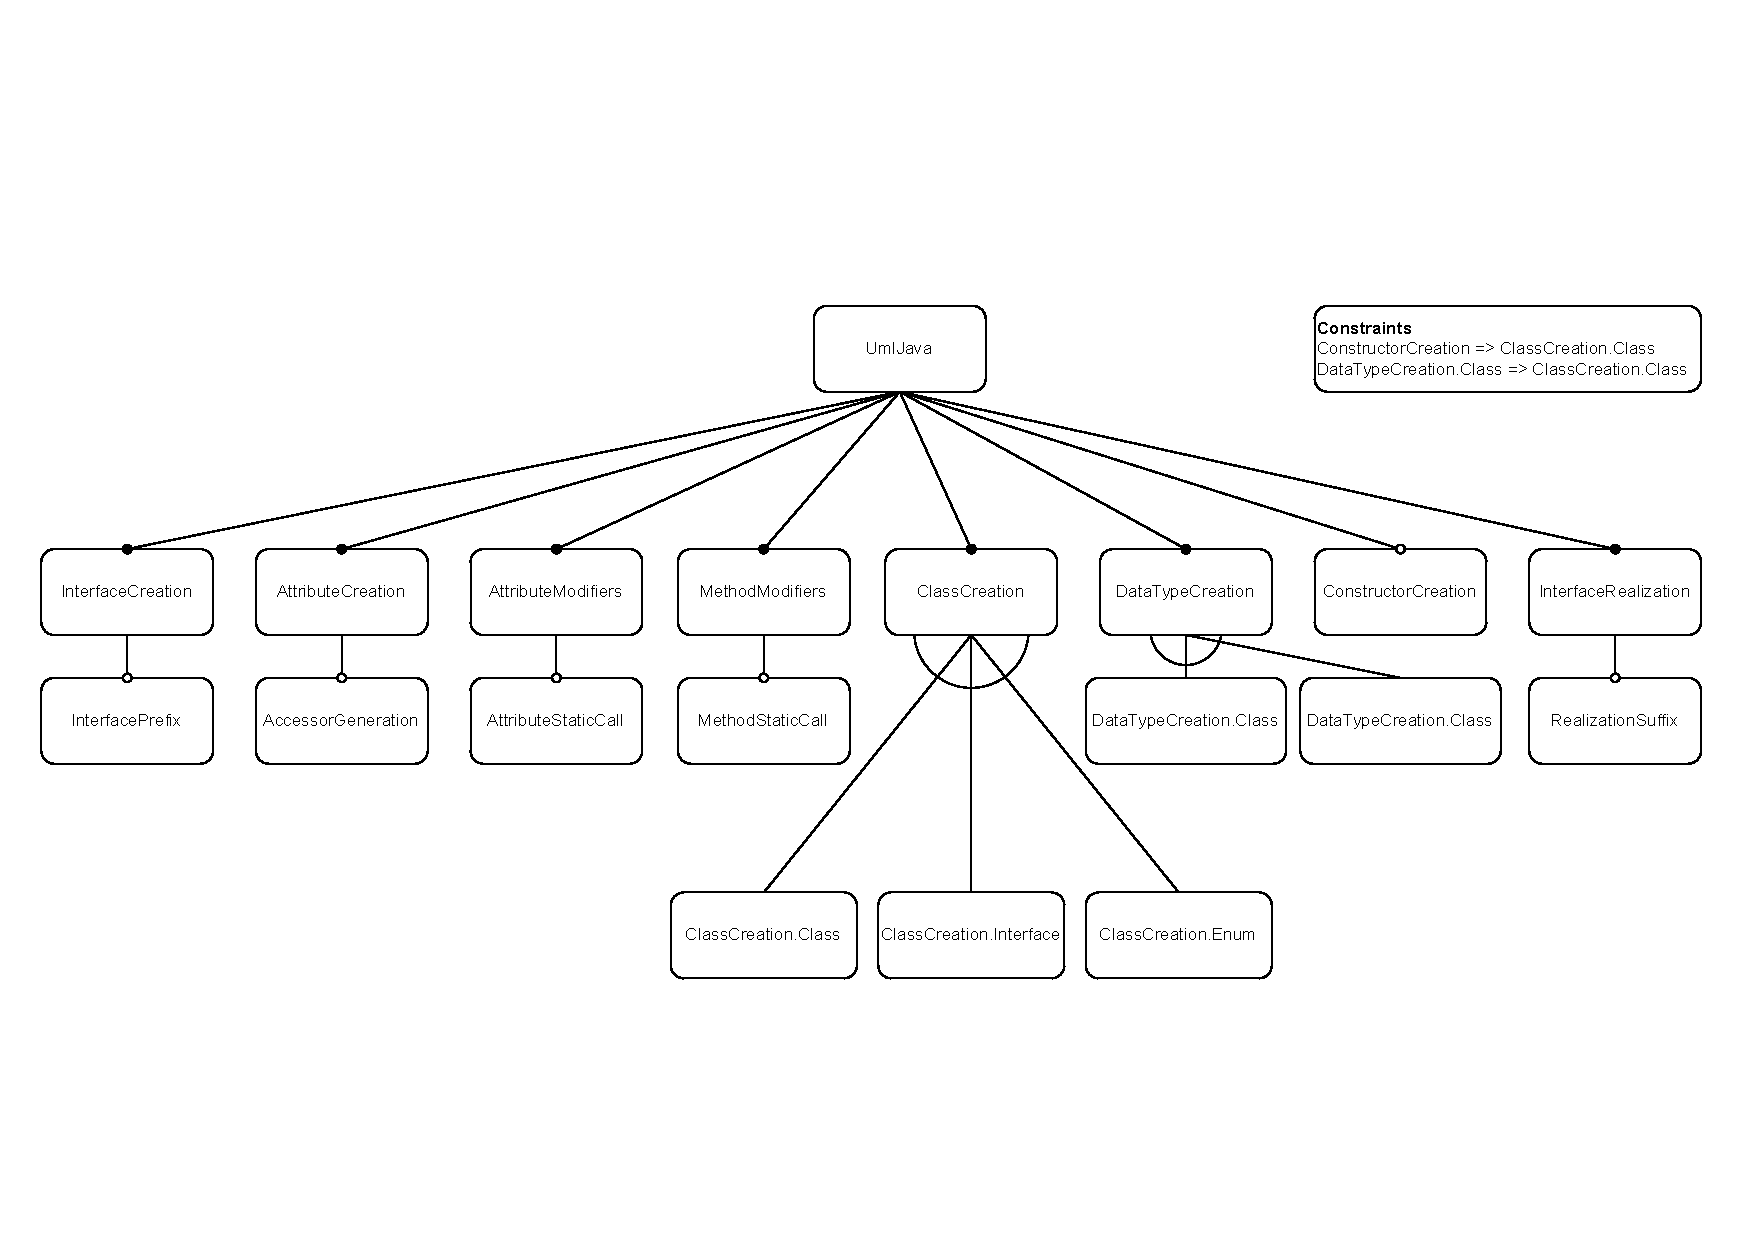
\includegraphics[width=\textheight, height=0.9\textwidth, keepaspectratio]{examples/library/reduced feature model.pdf}
    \caption{Reduced feature model}
    \label{fig:reduced-feature-model}
\end{sidewaysfigure}

Only a small subset is shown in \autoref{fig:reduced-feature-model}.
The excluded features are either mandatory or appear in every configuration, so it is not necessary to examine them more closely.
With the help of the feature model, nine configurations are extracted to represent all features at least once.
This allows each feature to be tested on its own.

\begin{table}[htbp]
    \centering
    \begin{tabular}{|l|c|c|c|c|c|c|c|c|c|}
        \hline
        \textbf{Feature}                 & \textbf{1} & \textbf{2} & \textbf{3} & \textbf{4} & \textbf{5} & \textbf{6} & \textbf{7} & \textbf{8} & \textbf{9} \\
        \hline
        \textit{Feature core}            & \checkmark & \checkmark & \checkmark & \checkmark & \checkmark & \checkmark & \checkmark & \checkmark & \checkmark \\
        \hline
        \textit{ClassCreation.Class}     & \checkmark & \checkmark & \checkmark & \checkmark & \checkmark & \checkmark &            &            & \checkmark \\
        \hline
        \textit{ClassCreation.Interface} &            &            &            &            &            &            & \checkmark &            &            \\
        \hline
        \textit{ClassCreation.Enum}      &            &            &            &            &            &            &            & \checkmark &            \\
        \hline
        \textit{DataTypeCreation.Class}  & \checkmark & \checkmark & \checkmark & \checkmark & \checkmark & \checkmark &            &            & \checkmark \\
        \hline
        \textit{DataTypeCreation.Record} &            &            &            &            &            &            & \checkmark & \checkmark &            \\
        \hline
        \textit{InterfacePrefix}         &            & \checkmark &            &            &            &            &            &            & \checkmark \\
        \hline
        \textit{RealizationSuffix}       &            &            &            & \checkmark &            &            &            &            & \checkmark \\
        \hline
        \textit{AccessorGeneration}      &            &            & \checkmark &            &            &            &            &            & \checkmark \\
        \hline
        \textit{ConstructorCreation}     &            &            &            &            & \checkmark &            &            &            & \checkmark \\
        \hline
        \textit{AttributeStaticCall}     &            &            &            &            &            & \checkmark &            &            & \checkmark \\
        \hline
        \textit{MethodStaticCall}        &            &            &            &            &            & \checkmark &            &            & \checkmark \\
        \hline
    \end{tabular}
    \caption{Features selected by the nine configurations. A checkmark marks a selected feature, and the feature core row stands for the 26 features every configuration selects.}
    \label{table:library-configurations}
\end{table}

\Autoref{table:library-configurations} lists the selected features by each of the nine configurations.
26 of the 37 features are selected in every configuration and form the core mapping between UML and Java.
These features cover the mapping of models, packages, names, visibilities, multiplicities, and primitive types, the creation and deletion of classes, attributes and methods, the creation of interfaces and enumerations, attributes, return and parameter types together with the direction of parameters.
They also cover class, attribute, and method modifiers, as well as inheritance, interface realization and the constraints of classes, interfaces, enumerations and parameters.
Like every other reaction, their reactions carry an annotation.
22 of these features are mandatory, so no valid configuration can drop them, whereas the four constraint features are optional but selected by all nine configurations.
Therefore, only the reactions of the remaining eleven features differ between two of the nine configurations.
Of those eleven features, only some are selected in each configuration.
\textit{ClassCreation} and \textit{DataTypeCreation} are alternative groups, so each configuration selects one of each, while the other features are optional.

The features from \autoref{fig:reduced-feature-model} have greater importance and require more information.
Their effects are shown in the classifiers of the library example in \autoref{sec:RunningExample:LibraryExample}, whose UML model is shown in \autoref{fig:library-example}.
\textit{InterfaceCreation} maps a UML interface to a Java interface in its own compilation unit, and vice versa.
Its optional child, \textit{InterfacePrefix}, prefixes the name of every interface with an \texttt{I} in both models, so \texttt{Borrowable} becomes \texttt{IBorrowable}.
Names starting with an \texttt{I} keep their original form, leaving \texttt{Identifiable} untouched.
\textit{AttributeCreation} maps UML properties to Java fields and vice versa.
With \textit{AccessorGeneration}, every attribute is made private and receives a getter and a setter.
These are renamed and deleted together with the attribute.
This turns \texttt{Media.title} into a private field with \texttt{getTitle} and \texttt{setTitle}.
\textit{AttributeModifiers} synchronizes the \texttt{final} and \texttt{static} modifiers of Java fields with the read only and static properties of UML attributes.
\textit{AttributeStaticCall} builds on that.
As soon as an attribute becomes static, its accessors become static as well.
Every access is rewritten as static access through the class.
Thus, the accessors of \texttt{LibraryCard.cardNumber} read and write \texttt{LibraryCard.cardNumber} instead of \texttt{this.cardNumber}.
Similarly, \textit{MethodModifiers} synchronizes the \texttt{abstract}, \texttt{final}, and \texttt{static} modifiers of Java methods with the abstract, leaf and static properties of UML operations.
Its optional child, \textit{MethodStaticCall}, works similarly to \textit{AttributeStaticCall}.
Furthermore, it turns the method \texttt{final}, which is a leaf operation in UML.
Consequently, the static \texttt{Member.register} becomes \texttt{static final}.
The function of \textit{ClassCreation.Class}, is to facilitate the mapping of a UML class to a Java class, and vice versa, in a manner consistent with the original reactions.
The new alternatives \textit{ClassCreation.Interface} and \textit{ClassCreation.Enum} realize every UML class as a Java interface or enum and every Java class as a UML interface or enumeration.
In the library example \texttt{Member} becomes an interface, with its attributes being designated as \texttt{static final} fields, or an enumeration without any literal.
\textit{DataTypeCreation.Class} maps a UML data type to a Java class, while the \textit{DataTypeCreation.Record} maps to a \texttt{final} Java class.
A final Java class is not extendable, a limit that also applies to \texttt{Isbn}.
It is not possible to establish a direct mapping to a Java record, as this functionality is not supported by \hyperref[sec:Foundations:JaMoPP]{JaMoPP}.
The \textit{InterfaceRealization} feature maps the interface realizations of UML classes to the \texttt{implements} references of Java classes, whenever one is added, removed, or replaced.
The optional child \textit{RealizationSuffix} functions similar to \textit{InterfacePrefix}, yet it appends \texttt{Impl} to a realization.
Consequently \texttt{Media} becomes \texttt{MediaImpl}.
Besides the four constraint features, the only optional feature located directly beneath the root element is \textit{ConstructorCreation}.
A public default constructor is appended to each new class, as an operation in UML and a constructor in Java.
The constructor is renamed, along with the class, resulting in the addition of a \texttt{Member()} constructor in \texttt{Member}.
The feature model introduces two additional constraints.
\textit{ConstructorCreation} and \textit{DataTypeCreation.Class} both require \textit{ClassCreation.Class}.

\section{Library example}
\label{sec:RunningExample:LibraryExample}

The process of obtaining measurements and the creation and interaction with a V-SUM necessitate a real example.
For the purpose of this study umljava is defined as a system that incorporates both a UML model and Java source code.
This integration enables the creation of a V-SUM with preprocessed reactions and can be migrated to different configurations afterward.
The example under consideration is a library with different types of media, interfaces with polymorphism, members, and all kinds of properties.
It is derived with the first configuration, which mirrors the behavior of the original reaction set.
The UML model for the first configuration is shown in \autoref{fig:library-example}.

\begin{figure}[htbp]
    \caption{Library example}
    \centering
    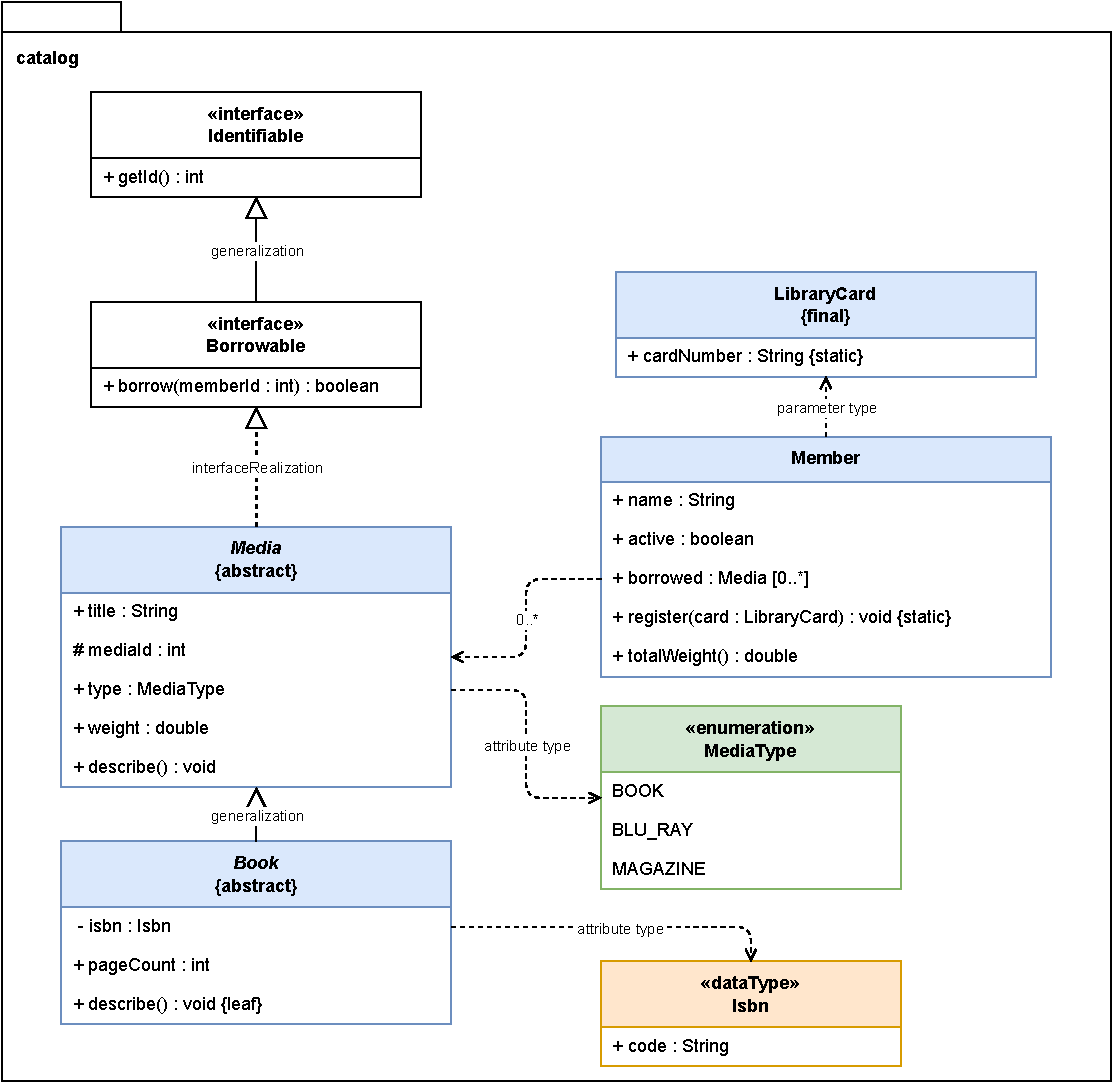
\includegraphics[width=\textwidth]{examples/library/library.pdf}
    \label{fig:library-example}
\end{figure}

All elements are contained within a single package \texttt{catalog} and consist of eight classifiers.
The interfaces \texttt{Identifiable} and \texttt{Borrowable}, the latter extends the former, and both declare the operations \texttt{getId} and \texttt{borrow}.
\texttt{MediaType} is an enumeration comprised of the literals \texttt{BOOK}, \texttt{BLU\_RAY} and \texttt{MAGAZINE}, while the \texttt{Isbn} data type is characterized by a single attribute \texttt{code}.
The abstract class \texttt{Media} carries the attributes \texttt{title}, the protected \texttt{mediaId}, \texttt{type} and \texttt{weight}.
It realizes \texttt{Borrowable} and declares \texttt{describe}.
The abstract \texttt{Book} extends it, and adds the private \texttt{isbn} and \texttt{pageCount}, in addition to a leaf \texttt{describe}.
\texttt{LibraryCard} is a final specialization holding the static \texttt{cardNumber}.
\texttt{Member} has the attributes \texttt{name}, \texttt{active} and \texttt{borrowed}, which holds zero to many \texttt{Media}, as well as the static operation \texttt{register} and the operation \texttt{totalWeight}.
Depending on the configuration that is selected, the V-SUM can accomodate between 216 and 437 model elements.
The least number of classifiers is observed in the seventh configuration, where classifiers become interfaces, that do not carry fields, accessors, or constructors.
The greatest number of classifiers is observed in the eighth and ninth configuration.

\lstinputlisting[frame=single, caption={Handwritten method body of \texttt{Member}}, label=listing:total-weight, numbers=left, float=htbp, language=Java]{examples/totalWeight.java}

While the rules derive the attribute \texttt{Media.weight} and the signature of \texttt{Member.totalWeight} from the UML model, the body shown in \autoref{listing:total-weight} has no counterpart there.
The method is composed of three statements, a local variable declaration, a loop over the borrowed media accumulating their weight, and a return.
This constitutes the sole instance of user written content in the given example, which serves as one criterion for evaluating the preservation of such content.